\documentclass{mipt-thesis-bs}
    % Следующие две строки нужны только для biblatex. Для inline-библиографии их следует убрать.
    %\usepackage{mipt-thesis-biblatex}
    %\addbibresource{bib.bib}

\title{Спектры предложений первого порядка с ограниченным количеством переменных}
\author{Ярмошик Д.\,В.}
\supervisor{Жуковский М.\,Е.}
%\referee{Петров Д.\,Е.}       % требуется только для mipt-thesis-ms
\groupnum{573}
\faculty{Факультет управления и прикладной математики}
\department{Кафедра «Интеллектуальные системы», специализация «Проектирование и организация систем»}

\begin{document}

\frontmatter
\titlecontents

\mainmatter

\chapter{Аннотация}
//TODO

\chapter{Введение}
    Случайные графы -- один из центральных разделов дискретной математики, расположенный на стыке теории вероятностей, комбинаторики и теории графов.
    Основы теории случайных графов были заложены в 50-х -- 60-х годах прошлого века венгерскими математиками П.~Эрдёшем и А.~Реньи.
    Существует множество моделей случайных графов, разработанных с учётом адекватности их применения в прикладных областях.
    В настоящей работе мы будем иметь дело с \textit{моделью Эрдёша-Реньи}, также называемой \textit{классической моделью} случайного графа.
    % Определение G(N,p)
    
    Многие вопросы этой теории связаны с асимптотическими свойствами случайного графа, то есть с тем, как он ведёт себя при устремлении количества вершин $N$ к бесконечности.
    Удивительным образом оказывается, что для целого класса таких вопросов можно, совершенно не вдаваясь в сущность конкретного вопроса, дать на него едва ли не исчерпывающий ответ.
    Точнее говоря, если про случайный граф спрашивается ,,Как, при увеличении числа вершин до бесконечности, будет вести себя вероятность того, что граф обладает свойством $A$?`` то во многих случаях можно заранее сказать: ,,Будет стремиться к 0 или к 1``.
    В этом состоит суть теорем, называемых \textit{законами нуля или единицы}, уточнению условий применимости которых посвящена данная работа.
    
    Чтобы перейти к изложению известных результатов о законах нуля или единицы, дадим определения основным понятиям и сформулируем теоремы, касающиеся важных для нас свойств случайного графа $G(N,p)$ (см. \cite{survey2015})
    
    Пусть $N \in \N$, $0 \leq p \leq 1$. Рассмотрим множество $\Omega_N = \{G = (V_N , E)\}$, $|\Omega_N| = 2^{C_N^2}$ всех неориентированных графов без петель и кратных ребер с множеством вершин $V_N = \{1, \ldots, N \}$.
    
    \Def \textit{Случайный граф $G(N, p) \in \Omega_N$  в модели Эрдёша-Реньи} -- это элементарный исход в вероятностном пространстве $(\Omega_N, P_{N.p}, 2^{\Omega_N})$, где  распределение $P_{N.p}$ определяется формулой $P_{N.p}(G) = p^{|E|}(1-p)^{C_N^2-|E|}$
    
    \Def Для произвольного языка $\F$ , случайный граф $G(N, p)$ \textit{подчиняется закону нуля или единицы для языка $\F$},
    если для любой формулы $\varphi$ из языка 
    $\F$  выполнено
    $\lim_{N \rightarrow \infty} P(G(N, p) \vDash \varphi) \in \{0, 1\}$.
    
    Введём обозначение $\LL$ для языка первого порядка с сигнатурой, в которую входят только двуместные предикаты равенства ($=$) и смежности ($\sim$).
    За точными определениями можно обратиться, например, к
    \cite{shen}, а здесь мы ограничимся лишь напоминанием о том, что формулы языка первого порядка -- это предложения, составленные из символов, обозначающих переменные: 
    $x,y,z,x_1,\ldots$, 
    логических связок 
    $\wedge, ~\neg, ~\vee$, 
    кванторов 
    $\exists, ~\forall$ и 
    предикатных символов (в нашем случае
    $\sim, ~ =$).
    Например, формула, утверждающая, что диаметр графа не превосходит 2, выглядит так:
    \[
    \forall x \forall y ~ x=y \vee x\sim y \vee \exists z ~ x \sim z \wedge z \sim y
    \]
    
    \Def \textit{Плотность} графа $G$ 
   \[ \rho_G = \frac {|E(G)|}{|V(G)|} \]
   
   \Def \textit{Максимальная плотность} графа $G$
     \[ \rho^{max}_G = \max_{H \subseteq G} \frac {|E(H)|}{|V(H)|} \]
    
    \Def Граф $G$ называется \textit{сбалансированным}, если 
    \[ \rho^{max}_G = \rho_G \]
    
    \Def Граф $G$ называется \textit{строго сбалансированным}, если 
    \[\rho^{max}_G = \rho_G > \max_{H \subsetneq G} \frac {|E(H)|}{|V(H)|} \]
     
В 1960 г. П. Эрдёш и А. Реньи
доказали теорему о об условиях справедливости утверждения “$G(N, p)$ содержит копию данного сбалансированного графа” \cite{erdHos1976evolution}. 
Позже этот результат получил следующее обобщение
    
\begin{theorem} (А. Ручински, А. Винс, 1985, \cite{rucinski1985balanced}) 
\label{th:ruchinski}
Вероятность того, что $G(N, p)$ имеет подграф $H$ стремится к 1 при $N \rightarrow \infty$, если $N^{-1/\rho^{max}(H)} = o(p(N))$ и стремится к  0, если $p(N) = o\left(N^{-1/\rho^{max}(H)}\right)$

\end{theorem}

Для нас очень важно то, что при $p = N^{-1/\rho^{max}(H)}$ вероятность содержать подграф $H$ не стремится ни к нулю, ни к единице.
Это утверждение, содержащееся в следующей теореме, даёт удобный способ доказывать отсутствие законов нуля или единицы для $G(N, N^{-\alpha}), ~\alpha \in \Q$

\begin{theorem} (Б. Боллобаш, 1981, \cite{bollobas1981threshold}). Пусть $H$~-- строго сбалансированный граф, $a$~-- количество автоморфизмов графа $H$, $p = N^{-1/ \rho^{max}_H}$
Тогда
\[N_H \xrightarrow[N\rightarrow \infty]{d} Poiss(1/a) \]
Здесь $N_H$ -- количество копий графа $H$ в $G(N, p)$, $Poiss(1/a)$ -- пуассоновская случайная величина со средним $1/a$.
\end{theorem}
Из последней теоремы и доказанного в \cite{rucinski1986strongly} утверждения о том, что для любого $\alpha \in (0,1] \cap \Q$ существует граф $H$ с плотностью $\rho_H = 1/\alpha$, следует, что $G(N,N^{-\alpha})$ не подчиняется закону нуля или единицы для языка $\LL$ при всех рациональных $\alpha$ из отрезка $[0,1]$.
Это верно и для $\alpha = (k+1)/k~, k > 0$, т.к. для каждого из таких $\alpha$ существует дерево с соответствующей плотностью.
При $\alpha > 2$ граф $G(N, N^{-\alpha})$ почти наверное пуст, и, следовательно, подчиняется закону нуля или единицы.
Оказывается, что при всех прочих $\alpha$ случайный граф $G(N, N^{-\alpha})$ также подчиняется закону нуля или единицы.
Итак, имеет место следующая теорема
\begin{theorem} (Дж. Спенсер, С. Шела, 1988, \cite{shelah1988zero})
Случайный граф $G(N, N^{-\alpha})$ подчиняется закону нуля или единицы для языка $\LL$ при всех $\alpha$, кроме $\alpha \in \left([0,1] \cap \Q \right) \cup \{(k+1)/k ~|~ k > 1\}$.
\end{theorem}

Ниже мы сформулируем несколько аналогичных теорем для других языков.

\Def Язык $\LL^k$ -- подмножество $\LL$, содержащее предложения, в которые входят не более $k$ переменных.

На языке $\LL^3$ для любого натурального $d$ можно выразить, например, свойство ``иметь диаметр не более $d$'': 
\[
\forall x \forall y ~ x = y \vee x \sim y \vee \left( \exists z ~ x\sim z \wedge z \sim y \right)
\vee  \left( \exists z ~ x\sim z \wedge \exists x ~ z \sim x \wedge x \sim y \right) \vee \ldots
\]

\Def Язык $\LL^k_{\infty, \omega}$ включает в себя предложения конечной или счётной длины, в которые входят не более $k$ переменных.

На языке $\LL^3_{\infty, \omega}$ можно выразить, например, свойство ``быть связным''.
Это свойство невыразимо в $\LL$.

\Def \[\LL^\omega_{\infty, \omega} = \bigcup_k \LL^k_{\infty, \omega} \]

\begin{theorem}
Случайный граф $G(N, N^{-\alpha})$ подчиняется закону нуля или единицы для языка $\LL^\omega_{\infty, \omega}$ при $\alpha \in (1,2] \setminus \{(k+1)/k ~|~ k > 1\}$ (Дж. Линч, 1993  \cite{lynch1993infinitary}) и $\alpha > 2$.
Закон нуля или единицы не выполнен при $\alpha \in [0,1]$ (С. Шела, 2017 \cite{shelah2017failure})  и $\alpha \in \{(k+1)/k ~|~ k > 1\}$.
\end{theorem}

\begin{theorem} (М. Mакартур, 1997 \cite{mcarthur1997asymptotic})
Для любых $\alpha < \dfrac{1}{k-1}$, $G(N, N^{-\alpha})$ подчиняется закону нуля или единицы для языка $\LL^k_{\infty, \omega}$.
\end{theorem}

\Def \textit{Кванторная глубина} формулы -- наибольшее число вложенных кванторов в формуле.

\Def Язык $\LL_k$ - подмножество $\LL$, включающее формулы с кванторной глубиной не более $k$.

\begin{theorem}(М. Е. Жуковский, 2012, [60]). Пусть $p=N^{-\alpha}$, $0 < \alpha < 1/(k - 2)$. 
Тогда случайный граф $G(N, p)$ подчиняется закону нуля или единицы для языка $\LL_k$.
\end{theorem}

\chapter{Постановка задачи}
Нас интересуют выразительные способности языков $\LL^k$ и $\LL^k_{\infty, \omega}$ и, в частности, наиболее простых среди них -- языков  $\LL^3$ и $\LL^3_{\infty, \omega}$.
Из результата Макартура следует, что для этих языков выполнен закон нуля или единицы при $\alpha < \frac{1}{2}$.
Кроме того, известно (М. Жуковский, А. Раджафимахатратра, 2019 \cite{razafimahatratra2019zero}), что при $\alpha = \frac{1}{k-1}$ закон нуля или единицы для языка $\LL^k$ всё ещё справедлив, но в любой правой полуокрестности $\frac{1}{k-1}$ существует $\alpha$, для которого закон нуля или единицы нарушается.
Что можно сказать о сохранении закона нуля или единицы для языков с тремя переменными при других значениях параметра $\alpha$, например в окрестности $\alpha=1$ -- точки, при переходе через которую граф теряет связность?
Существуют утверждения, не выразимые на языке $\LL$, но выразимые в $\LL^3_{\infty, \omega}$ и наоборот.
Для языка $\LL$ закон нуля или единицы выполнен при всех иррациональных $\alpha$, верно ли это для $\LL^3_{\infty, \omega}$?
Различается ли структура множеств параметров, на которых нарушается закон нуля или единицы, у языков с ограниченным количеством переменных и языков с ограниченной кванторной глубиной? 

\chapter{Доказательства теорем}
\section{Формула из $\LL^3_{\infty, \omega}$ с бесконечным спектром}

\Def \textit{Спектром} формулы $\varphi$ называется множество $\alpha$ таких, что вероятность $P\left( G\left(N, N^{-\alpha}\right) \vDash \varphi  \right)$ не стремится ни к 0, ни к 1 при $N \rightarrow \infty$.
Здесь использовано обозначение $G \vDash \varphi$, означающее, что для графа $G$ справедливо $\varphi$.

\begin{theorem}
В языке $\LL^3_{\infty, \omega}$ существует формула с бесконечным спектром с предельной точкой 1 (справа).
\end{theorem}
\begin{proof}
Обозначим $\varphi_m$ замкнутую формулу, которая истинна тогда и только тогда, когда в графе существует цикл длины не более $m$  или простой путь длины $m$,  $\varphi_m \in \mathcal{L}^3$. Например,
\[
\varphi_3 = \exists x ~\exists y ~
 x \sim y  \wedge \left( \exists z ~ y \sim z \wedge  z \neq x 
\wedge \left(\exists x ~ x \sim z \wedge x \neq y
\right) \right) 
\]
%\textstyle\bigwedge\limits
Определим $\varphi \in \mathcal{L}^3_{\infty, \omega}$ :
\[
\varphi = \bigvee_{k = 2}^{+\infty}\left(
\wedge_{i=3}^{2k-1} \varphi_{i}  \wedge \neg \varphi_{2k} \right)
\]

Пусть $\alpha = 1 + \frac{1}{2k}$.
Напомним, что при таком $\alpha$, по теореме \ref{th:ruchinski}, вероятность обнаружить в случайном графе $G(N, N^{-\alpha})$ подграф $H$ с плотностью $\rho_H > \frac{2k}{2k+1}$ стремится к нулю, с плотностью $\rho_H < \frac{2k}{2k+1}$ стремится к 1, а с плотностью $\rho_H = \frac{2k}{2k+1}$ -- ни к нулю ни к единице.
Поскольку $\frac{2k}{2k+1}$ -- это плотность простого пути длины $2k$, то асимптотически почти наверное случайный граф $G(N, N^{-\alpha})$ содержит простой путь длины $2k-1$ , поэтому в формуле $\varphi$ дизъюнкция конъюнктов до $k-1$ -го включительно ложна с вероятностью, стремящейся к 1.
Также, с вероятностью, стремящейся к 1, $G(N, p)$ не содержит циклов длины не более $2k+1$ и простых путей длины $2k+1$.
Поэтому дизъюнкция конъюнктов от $k+1$-го до бесконечности ложна с вероятностью, стремящейся к 1.

Количество простых путей длины $2k$ в $G(N, N^{-\frac{2k+1}{2k}})$ имеет асимптотическое распределение $Poiss(1/2)$, поэтому
$$
P(G(n, p) \models \varphi) = 
P(G(n, p) \models \neg \varphi_{2k}) \rightarrow e^{-1/2}
$$

Аналогично, при $\alpha = 1 + \frac{1}{2k+1}$ 
$$P(G(n, p) \models \varphi) = 
P\left(G\left(n, p \right) \models  \varphi_{2k+1}\right) \rightarrow 1 - e^{-1/2}$$

Таким образом, спектр формулы $\varphi$ содержит множество $\{1 + 1/k ~|~ k > 5 \}$, что и требовалось.
\end{proof}

\section{Предельные точки $\LL^3$ в левой окрестности единицы}
\Def Назовём \textit{предельной точкой} такое $\alpha$, что в любой окрестности $\alpha$ существует $\alpha'$, для которого не выполнен закон нуля или единицы.

Докажем, что в языке $\mathcal{L}^3$ предельные точки существуют в любой левой полуокрестности единицы: 
$\forall \varepsilon > 0 ~ \exists \alpha \in (1 - \varepsilon, 1)$.

Рассмотрим граф, состоящий из $k+2$ треугольников, соединённых простыми путями.
Причём, расстояние (в рёбрах) между вторым и третьим треугольниками, третьим и четвёртым и т. д., одинаково.
Обозначим это расстояние $m$, а расстояние между первым и вторым треугольником - $s$.

\begin{figure}[h]
    \centering
  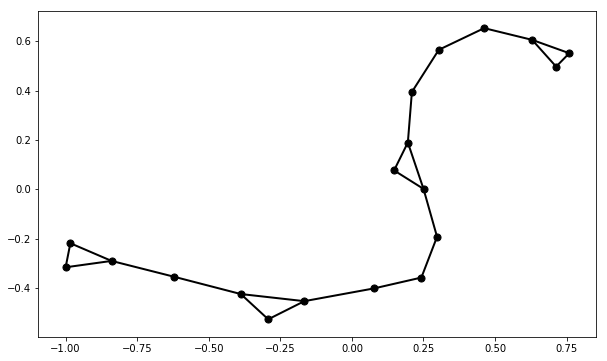
\includegraphics[scale=0.4]{picrel/index.png}
  \caption{Граф с $k = 2$, $s = 2$ и $m = 4$}
  \label{fig:chain1}
\end{figure}

Плотность такого графа равна 
$$\rho_{H_{ksm}} = \dfrac{6+s + (3+m)k}{5+s + (2+m)k}$$
и при увеличении $k$ стремится к $\rho_\infty = \dfrac{3+m}{2+m}$.

Граф с $k=0$ состоит из двух треугольников и имеет вид гантели.

Т.к. 
$sign\left(\dfrac{\partial\rho_{H_{ksm}}}{\partial k}\right) = sign(3+s-m)$,
то при $m < 3 + s$ плотность графа растёт при увеличении  $k$ и, как нетрудно убедиться, при этом выполнено равенство
$\rho_{H_{ksm}} = \rho^{max}_{H_{ksm}}$.
Будем считать $m = s+2$, т.к. при таком соотношении длины гантели и длины добавочных звеньев
граф получается оптимальным с точки зрения плотности, что пригодится в дальнейшем.

Таким образом, для доказательства утверждения достаточно предъявить для каждого такого графа формулу из  $\mathcal{L}^3$, выражающую его существование.

Вместо 
$\exists x \exists y \exists z ~ x \sim y \wedge y \sim z \wedge x \sim z$
будем писать 
$\exists x~\triangle_{xyz}$

Формула, выражающая существование гантели, имеет вид:
\def\gantelRightPart {
&\wedge \exists x ~ 
    \left[ x \sim z \wedge x \neq y \wedge x \nsim y  \right] \\
&\wedge \exists y ~
    \left[ y \sim x \wedge y \neq z \wedge y \nsim z \right] \\
&\wedge \exists z ~
    \left[ z \sim y \wedge z \neq x \wedge z \nsim x  \right] \\
&\wedge ~ \qquad \qquad \cdots \\
&\wedge \exists x ~ 
    x \sim z \wedge x \sim y
}

\begin{equation}
\label{f:gantel}
\begin{split}
\exists x~\triangle_{xyz} \gantelRightPart,
\end{split}
\end{equation}
где количество выражений в квадратных скобках равно числу вершин между треугольниками минус 2

Формула $\varphi_{ksm} $, выражающая существование графа $H_{ksm}$, выглядит аналогично, только часть формулы (\ref{f:gantel}), следующая за 
$\exists x~\triangle_{xyz}$,
содержит $s-1$ выражение в квадратных скобках и повторяется ещё $k$ раз, и каждая из повторяющихся частей содержит $m-1 $ выражение в квадратных скобках.
% \begin{equation}
% \label{f:phiKsm}
% \left. 
%     \begin{split}
%         \exists x~\triangle_{xyz} 
%         \gantelRightPart
% \right\}
% \left. 
%     \left. \gantelRightPart \right\}
%     \left. \gantelRightPart \right\}
% \right\}
% \end{equation}

% \[
% \begin{split}
% \left.
% a = b \\
% c = d
% \right\}
% \end{split}
% \]

Конечно, вообще, существование в $G(n, n^{-\alpha})$ подграфа $H_{ksm}$ не является необходимым для того, чтобы формула $\varphi_{ksm}$ была верна.
Однако, оно становится необходимым при $\alpha = 1/\rho_{H_{ksm}}$ и $m = s+2$. 
Действительно, покажем, что любой другой граф $\tilde H_{ksm}$, для которого выполнено $\varphi_{ksm}$, имеет максимальную плотность большую, чем $\rho_{H_{ksm}}$.

\begin{Lem} 
\label{lem:min_ro_Hksm}
Граф $H_{ksm}$ имеет минимальную $\rho^{max}$ среди всех графов, для которых выполнено $\varphi_{ksm}$
\end{Lem}

\begin{proof}
В графе $H_{ksm}$ каждой переменной формулы $\varphi_{ksm}$ соответствует отдельная вершина.
Любой другой граф $\tilde H_{ksm}$ либо получается путём добавления рёбер в $H_{ksm}$ (в этом случае увеличение плотности очевидно), либо имеет вершину, которой соответствует более одной переменной.
Далее будем рассматривать только второй случай.
Пусть в звене под номером $k'$ (номер $0$ соответствует гантели), впервые произошло повторное ``использование'' вершины. 

Более строго $k'$ можно определить так:

Равенство
$\varphi_{ksm}(\tilde H_{ksm}) = 1$
означает, что существует такая сюръекция из множества вершин графа во множество переменных формулы, что если в формулу вместо переменных подставить соответствующие вершины, получится верное утверждение.
Зафиксируем это соответствие.
Для каждого $k' < k$ определим $\tilde H'_{k'sm}$ как подграф $\tilde H_{ksm}$, индуцированный на множество вершин, соответствующее переменным, входящим в подформулу формулы $\varphi_{ksm}$, совпадающую с $\varphi_{k'sm}$.
Пусть теперь $k' \in $ такое, что в $\tilde H_{k'sm}$ есть вершина, которой соответствуют две переменные, а (если $k' \neq 0$) в $~\tilde H_{k'-1,sm}$ таких вершин нет.\\
$e:= e(H_{k'sm})$ , $v:= v(H_{k'sm})$\\
$\tilde e:= e(\tilde H_{k'sm})$ , $\tilde v:= v(\tilde H_{k'sm})$\\
Есть три возможности:
\begin{enumerate}
\item 
Последняя вершина в звене уже была использована - та, которая сразу добавляет два ребра
\begin{enumerate}
\item 
повторно использована только она: $\tilde \rho^{max} \geq \dfrac{e}{v-1}$ \\
В этом случае число вершин в $\tilde H_{k'sm}$ равно $v-1$, а число рёбер не меньше $e$. Действительно, в рассматриваемом случае (по определению) $\tilde H_{k'sm}$ содержит все рёбра $H_{k'sm}$, кроме, быть может, двух рёбер, инцидентных последней вершине, которые могут уже присутствовать в $H_{k'sm}$
Однако, легко видеть, что это невозможно (см. Рис. \ref{fig:only last reused}).
\begin{figure}
  \centering
  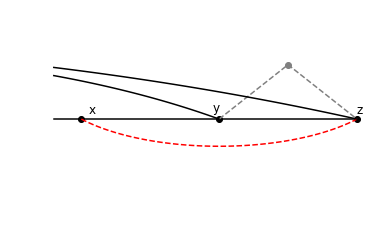
\includegraphics[scale=0.5]{picrel/only_last_reused.png}
  \caption{Только последняя вершина использована повторно. Черным обозначены вершины и рёбра $\tilde H_{k'sm}$, серым вершины и рёбра  $H_{k'sm}$, красным пунктиром - рёбра, запрещённые формулой  }
  \label{fig:only last reused}
\end{figure}
\item
она и какая-то до неё: $\tilde \rho^{max} \geq \dfrac{e-2}{v-2}$ \\
\begin{figure}
  \centering
  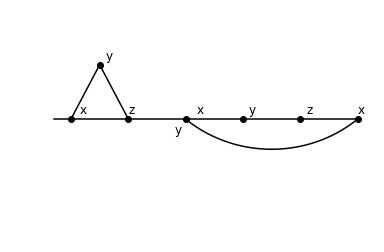
\includegraphics[scale=0.5]{picrel/reuse_intermediate.png}
  \caption{Повторное использование промежуточной вершины}
  \label{fig:reuse intermediate}
\end{figure}
\label{enum:reuse intermediate}
Посмотрим на первую повторно использованную вершину.
Т.к. формула запрещает совпадать вершинам, соответствующим разным переменным, для её соединения с предыдущими вершинами необходимо добавить ребро, которого нет в графе $H_{k'sm}$. 
С каждой новой секцией в $H_{k'sm}$ добавляется $3+m$ рёбер  и $2+m$ вершин.
Однако, проведя дополнительное ребро к уже имеющейся вершине, мы уже добавили на одно ребро больше, чем вершин, поэтому имеем рёбер $ e - (3+m) + (\nu+1) = e - (m-\nu) $, вершин $v - (2+m) + \nu = v - (m-\nu)$, где $\nu$ - число вершин, уже добавленных в последней, ,,секции'' $\tilde H_{k'sm}$.
Поскольку $\tilde H_{k'sm}$ связен, при добавлении новой вершины добавляется и как минимум одно ребро.
В рассматриваемом случае $\tilde v \leq v-2$, поэтому $\tilde \rho^{max} \geq \frac{e-2}{v-2}$ 
\end{enumerate}
\item
Последняя вершина ещё не была использована:
$\tilde \rho^{max} \geq \dfrac{e}{v-1}$\\
Случай похож на \ref{enum:reuse intermediate}, но теперь $\tilde v \leq v-1$ и последняя вершина добавляет 2 ребра
\end{enumerate}

Итого 
$\tilde \rho^{max} \geq \dfrac{e-2}{v-2} = \dfrac{4+s +(3+m)k'}{3+s + (2+m)k'}$. 

Используя $m=s+2$, получаем $\tilde \rho - \rho_\infty = \dfrac{1}{((2+m)(k+1)-1)(m+2)}$, следовательно
$\tilde \rho^{max} > \rho_\infty > \rho_{H_{ksm}} $.
\end{proof}

Из теоремы \ref{th:ruchinski} и леммы \ref{lem:min_ro_Hksm} следует следующий результат

\begin{theorem}
 Закон нуля или единицы для языка $\LL^3$ нарушается в точках $\alpha = \frac{m+3 + (2+m)k}{m+4 + (3+m)k}$, $m \geq 3$, $k \geq 0$.
В языке $\LL^3$ есть предельные точки в любой левой полуокрестности единицы.
\end{theorem}

\section{О законе нуля или единицы при иррациональных $\alpha$ для языка $\LL^3_{\infty, \omega}$}
Последовательность графов, у которых $\rho^{max}$ стремится к иррациональному числу, можно использовать для доказательства отсутствия закона нуля или единицы при рациональных $\alpha$.

Рассмотрим граф
\begin{figure}[h]
  \centering
  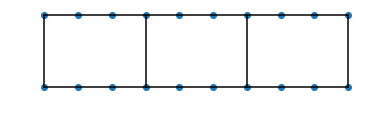
\includegraphics[scale=0.5]{picrel/first_block.png}
  \caption{Первый блок}
  \label{fig:first block}
\end{figure}

Если присоединить к нему кусочек, как на рисунке \ref{fig:2 blocks}, то плотность и максимальная плотность графа не изменятся

\begin{figure}[h]
  \centering
  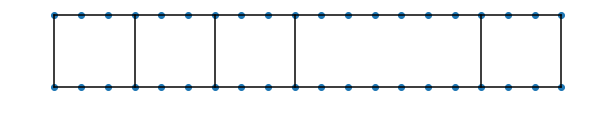
\includegraphics[scale=0.5]{picrel/2_blocks.png}
  \caption{Два блока}
  \label{fig:2 blocks}
\end{figure}

Можно присоединить 9 кусочков, увеличив число рёбер и 
вершин в десять раз, затем добавить (или не добавлять) одно ребро. Получившийся граф будет иметь вид, как граф на рисунке \ref{fig:additional edge}

Таким образом можно увеличивать число рёбер и вершин в $10^k$ раз и добавлять ребро.
Последовательность плотностей графов будет стремиться к бесконечной апериодической десятичной дроби.

\begin{figure}[ht]
  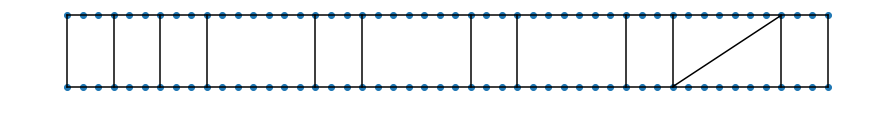
\includegraphics[scale=0.5]{picrel/additional_edge.png}
  \caption{Несколько блоков и дополнительное ребро}
  \label{fig:additional edge}
\end{figure}

Граф состоит из примыкающих друг к другу секций, поэтому для записи формулы, выражающей существование этого или более плотного графа, достаточно столько переменных, сколько нужно, чтобы выразить существование наибольшей из секций. 

//TODO: исправить -- приближаться к иррациональному числу нужно справа а не слева, рёбра нужно удалять, а не добавлять

\chapter{Заключение}
//TODO

\backmatter
\bibliographystyle{unsrt}
\bibliography{bib}

\end{document}